%
% Memory based reasoning - Project
% Specification
%
% created: 04. March 2012
%
\documentclass[11pt]{article}
\usepackage[T1]{fontenc}

% not needed here:
\usepackage{graphicx}
%\usepackage{hyperref}
%\hypersetup{
%    colorlinks,
%    citecolor=black,
%    filecolor=black,
%    linkcolor=black,
%    urlcolor=black
%}

% all the texturing effect
% sponge
% snapshot
% implementation details, diagramms, coefficients
% results of fiddeling with parameters

\usepackage{url}

\title{
	\emph{A Report for}\\
	\huge{\textbf{Soft Object Modelling \& Rendering} }\\
	-Project-\\
	Computer Graphics\\[2em]	
}
\author{
	Philipp Fonteyn (MS11F010)\\
	Paul Pellegrini (CS11F001)\\[2em]
	%\emph{Master of Technology}\\
	\emph{Computer Science \& Engineering, IIT Madras}
}
\date{20th of April 2012}

%
% Document
%
\begin{document}
\maketitle
\newpage
\tableofcontents
\newpage

%
%
%
\section{Introduction}
In modern computer science the field of computer graphics has gained much impulse due to faster performing devices, better and quicker memory access times and of course more efficient methods of algorithmic computation. Thus more and more realistic and complex scenes can be rendered by computational means and finally displayed on digital devices. This project will give a small overview over the technique of "soft modeling".
%
%
%
\section{Modeling Soft Objects}
When modeling the world solid objects such as e.g. a cube have clearly defined static shapes and appearance in the three-dimensional space. So called "soft objects" on the other hand are more flexible and can take various shapes and forms. Storing softer objects and their interaction with their surroundings needs therefore more thought as the solids.\\[1em]
%
There have been several models developed for modeling soft objects. The following paper will focus on the spring model approach described by \cite{LSCS} and \cite{hair}\cite{gama}.\\[1em]
%
\subsection{Spring}
A spring is a mechanical device, that is able to store and release kinetic energy. With given material properties a spring can be bent and twisted, then kept in this state until the bending force is released and the spring will return to its original state. As a mathematical approximation of the real world spring there is the very simple rule called \textit{Hooke's law}:
$$F=-kx$$
Where the force $F$ existing between the two ends of the spring is equal to the difference of displacement $x$ from its original state into a material or force constant $k$. If a spring is changed in its length, then at the both ends a mass $m$ will be moved with the acceleration $a$:
$$-kx = ma$$

\subsection{Spring Model}
In the so called spring model objects are modeled in such a way, that the respective mass points of the object are connected by springs. From the formula above one can imagine the behavior of the spring. If one point is moved due to an external force, it creates a force within the spring, which will pull it back to its original state.

\subsection{Wireframe}
In the wireframe representation of an object we can see where appropriate masspoints are. Edges between these points can be drawn and considered either as a plain edge (e.g. for visual effects) or as a spring, as above. Depending on how many springs and which distribution of mass points we use in an object different forces will be present and convey different stability and behavior to the object if forces are applied.
%
%
%
\section{Algorithm}
As algorithm we simply use the formula described above. After computing the internal forces of a spring it applies these forces to its mass points. Each mass point will sum up all forces pressing it and therefore with a certain acceleration move over a distance specified by acceleration into time-difference since last frame. These computations are repeated for each time-step.

\section{Work Done}
\subsection{Spring}
A simple spring consists of two mass points at each end. If we position the spring in a horizontal plane and apply a force downwards on one end, the length of the spring will increase and internally the spring will compute a inward bound force, which pulls the string back to his original length. Has the spring reached his original length, the movement pulling it back has not vanished and the spring will compress, hence yielding a relaxing force again. To prevent movement until infinity we add a dampening constant which will slowly bring the contraction-expansion cycle to an end.
\subsection{Rope}
By simply chaining up several springs, one can create a soft object which will behave like a rope. With four to six segments and a fixed endpoint the rope develops a realistic behavior under the influence of gravitational down-pull. To enhance the viewers experience we paint a textured GLUT cylinder around the single elements of the spline.

\subsection{Cloth}
After successful implementation of one-dimensional Spring-Model objects, we arrange the springs in a two-dimensional grid/net structure. Figure \ref{fig:cloth-grid} shows the arrangement of the springs shortly after the gravitation starts pulling the net to a great extend simulating a very flexible material. To achieve a more "stable" cloth we add diagonal connections between diagonal adjacent mass points, too. In order to visualize the cloth, for each rectangle of the gridmesh we draw two adjacent triangle polygons. This is following the approach of three-edged polygons, that is used in the wireframe model of many surfaces and objects. As not each material is so flexible like rubber, the spring coefficient can be increased to gain a stiffer cloth. Figure \ref{fig:cloth-stif} shows to cloth with different spring stiffness and an applied texture.

\begin{figure}[h]
\centering
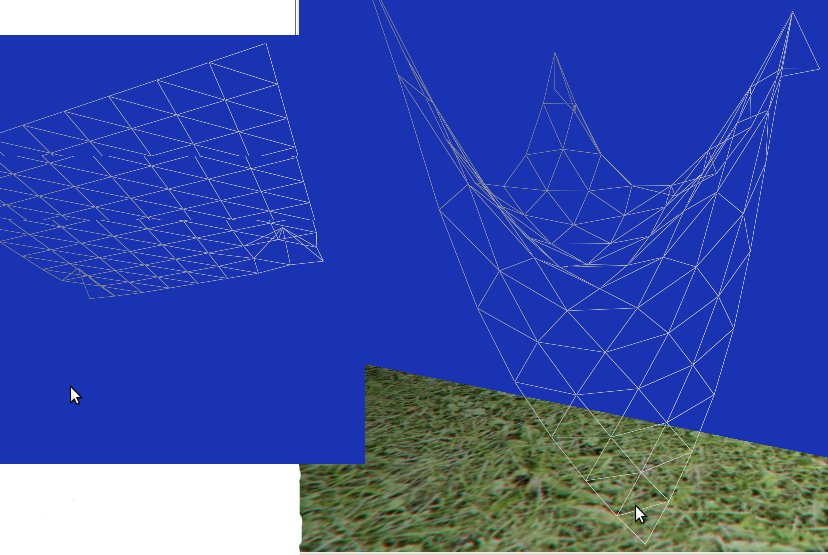
\includegraphics[scale=0.3]{cloth-grid.jpg}
\caption{Cloth wireframe a) shortly after initialization b) after effect of gravitation}
\label{fig:cloth-grid}
\end{figure}

\begin{figure}[h]
\centering
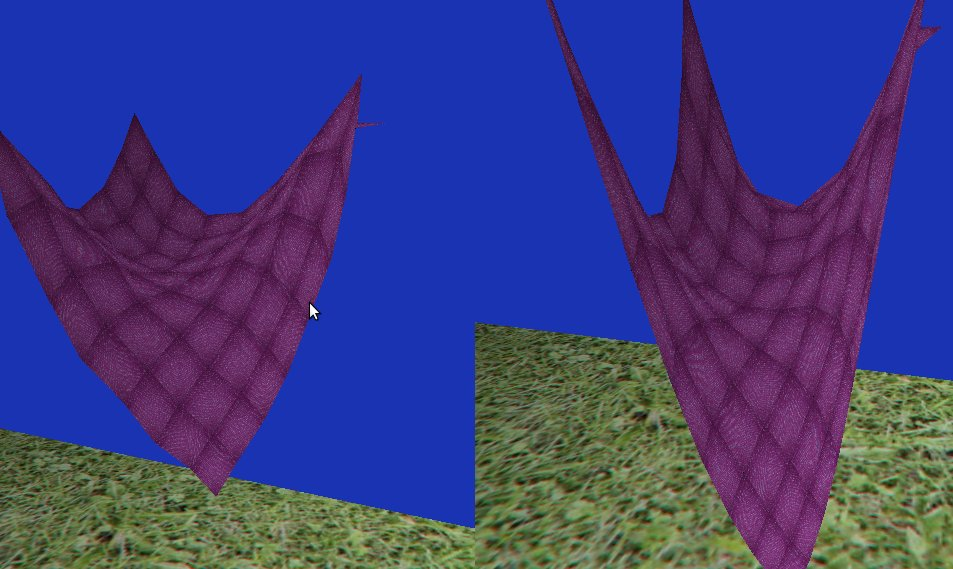
\includegraphics[scale=0.3]{cloth-stiffness.jpg}
\caption{Cloth with texture a) left stiff cloth b) right a flexible cloth}
\label{fig:cloth-stif}
\end{figure}


\subsection{Jelly}
The last dimension is demonstrated with a soft object which actually has a volume. We arrange our springs in a three-dimensional grid/cube. The behavior of the cube looks not very realistic, because the volume can actually implode. We countered this "collapsing"-effect with springs within the volume itself to enhance stability, which is not guaranteed by springs only placed on the surface of the object.
\subsection{Rendering}
Using the OpenGL framework for C++ we implemented a visualization of the effects described above. With texturing and lighting the soft objects we achieve a realistic scene.
%z depth buffer\\
%textureing\\
%camera\\
%fog
\subsection{Problems}
One problem we encountered during the implementation is the sudden "explosion" of the spring grid. We had to adjust the force constants within the springs to prevent this from happening. Due to our non-continuous calculation of spring forces, the forces existing in the spring itself may converge quickly shifting to $-\infty$ and $\infty$ -from one extreme to the other.\\[1em]
We can not calculate the forces in a continuous manner, because we actually have two sorts of time measures in our system. For one part there is the (virtual) \textit{physical world time} and the hardware induced \textit{frame refresh rate}. They are not in sync and therefore produce this asymmetry.\\[1em]
Finding the right constant for the spring constant and the mass points actual mass is therefore important for realistic simulation (or a super fast realtime displaydevice and graphics processor).
%
\section{Results}
The main objectives of the project are solved:
\begin{itemize}
\item{Usage of wireframe to model objects}
\item{then use of spring model to provide softness}
\item{then rendering using OpenGL}
\item{Effects of stress shown by physical forces such as gravity and wind}
\end{itemize}

\textit{Outlook for the project:}\\
With advanced time measuring methods the physical frame rate should be adapted to the graphical frame rate. Since our computations on the objects are functions of time $\Delta t$ the painting which is done by the OpenGL framework is a function of the speed of the graphics processor and displaying device (measured in $frames-per-second=fps$). Due to different $fps$ on different devices the physical framerate has to be adjusted to fit what the eye is seeing to improve the smoothness of the animation.\\[1em]
%
% Addition of FOG and COllision Detection ??

\section{Conclusion}
With a very simple physical equation the Spring Mass Model achieves a very realistic behavior of objects. If we work with more advanced models, with denser wireframes or within-springs with different hardness, even more advanced objects can be modeled. Since the Wireframe approach to model objects in computer graphics is very vastly present the Spring Mass Model is quite handy, since it can be easily put onto an existing wireframe, additional springs maybe added though to keep the object solid, otherwise it would simply collapse into itself.
%


%
% Literature / References
%
\newpage
\nocite{hill}
\nocite{rogersadams}
\nocite{dam}
\nocite{PBDM}
\nocite{baker}
\nocite{bakerGL}
\nocite{IASDO}
\nocite{LSCS}
\nocite{DCMSM}
\nocite{gama}
\nocite{wiki}
\nocite{hair}
\nocite{pyGL}
%\nocite{}
\bibliographystyle{alpha}
\bibliography{gc-bib}

%
% End of File
%
\end{document}
